% main.tex — arXiv preprint of P4-SHORT
% Cross-Family LLM-Judge Agreement for Institutional RAG
% Adisak Sukul, Iowa State University
% Build: pdflatex main && bibtex main && pdflatex main && pdflatex main

\documentclass[11pt,letterpaper]{article}

\usepackage[T1]{fontenc}
\usepackage[utf8]{inputenc}
\usepackage{lmodern}
\usepackage[margin=1in]{geometry}
\usepackage{graphicx}
\usepackage{booktabs}
\usepackage{array}
\usepackage{microtype}
\usepackage{textcomp}
\usepackage{amssymb}
\usepackage[hidelinks]{hyperref}
\usepackage[round]{natbib}
\usepackage{xcolor}

% Compact section headings
\usepackage{titlesec}
\titlespacing*{\section}{0pt}{1.4ex}{0.6ex}
\titlespacing*{\subsection}{0pt}{1.0ex}{0.4ex}

\graphicspath{{figures/}}

\title{\bfseries Cross-Family LLM-Judge Agreement\\ for Institutional RAG: \\ A 5-Family, 9-Judge Ablation}

\author{Adisak Sukul \\
  \small Iowa State University \\
  \small \texttt{asukul@iastate.edu}}

\date{2026-04-28}

\begin{document}
\maketitle

\begin{abstract}
\noindent\textbf{Open-weight LLM judges win the within-pair race.} In our 5-family, 9-judge LLM-as-Judge ablation on \textbf{570 RAG query--document pairs from an institutional repository}, the highest pairwise quadratic-weighted Cohen's $\kappa$ (0.80) is between Qwen 3.6 Plus and Gemma 4 26B---a cross-organization open-weight pair that exceeds every commercial within-family pair (Anthropic 0.71, OpenAI 0.63, Google-commercial 0.67) and ties the cross-family commercial reasoning ceiling. We present the first \textbf{five-family} pairwise $\kappa$ matrix on bounded 0--3 ordinal relevance with \textbf{four within-family controls} and report (i) cross-family reasoning judges converge at $\kappa = 0.75$--$0.79$; (ii) within-family agreement is task-dependent and bounded by the cross-family ceiling, contradicting canonical self-preference findings under bounded ordinal judging; (iii) two emergent calibration clusters (reasoning-generous vs.\ strict-mid) partition judges more cleanly than provider family. Mechanistic decomposition (companion long version) attributes \textbf{93\% of $\kappa$ variance to joint-distribution structure of paired scores}; structural factors (provider, reasoning-mode) are fully mediated; the shared-tokenizer hypothesis is refuted (Qwen$\leftrightarrow$Gemma vocabulary Jaccard $= 0.066$, lowest in slate, yet matrix-highest $\kappa$). External validation against \textbf{NIST TREC RAG 2024 human qrels} on a 537-pair stratified-balanced sample reaches 9-judge ensemble \textbf{$\kappa = 0.4941$} (Landis--Koch moderate, near-substantial); 5 of 9 individual judges hit $\kappa \geq 0.47$. We open-source \texttt{eval\_llm\_judge.py} and \texttt{validate\_against\_trec.py} (5,130 within-corpus + 4,833 external score records, USD~56.30, $\sim$13~hours wall) as reproducibility artifacts.
\end{abstract}

\section{Introduction}\label{sec:intro}

Modern RAG systems sit on top of vector retrievers tuned over institutional corpora---academic libraries, parliamentary archives, medical records, legal collections. Practitioners want to answer ``is this retrieval good?''---but they hit three blockers: there is no gold relevance set (TREC-style ground truth is prohibitively expensive), generic IR benchmarks (BEIR, MS-MARCO) do not transfer, and the canonical workaround---LLM-as-Judge \citep{zheng2023judge,faggioli2023perspectives,rahmani2024judges,upadhyay2024umbrela}---surfaces a new question: \emph{which} LLM judge?

The literature splits into camps. LLM-as-Judge advocates argue a frontier reasoning model is sufficient. Bias skeptics document position, verbosity, and self-preference biases \citep{wang2023fair,saito2023verbosity,panickssery2024self}, advocate ensembling, and call for meta-evaluation \citep{thakur2024judges}. RAG-eval frameworks \citep{es2024ragas} provide infrastructure but report agreement only against humans, not pairwise across LLMs. \textbf{No published paper, to our knowledge, reports pairwise quadratic-weighted Cohen's $\kappa$ across three or more model families on a bounded ordinal relevance rubric at $\geq 500$ paired observations, with within-family controls and open-weight peers as first-class judges.} Open-weight judges are the default for sovereign-cloud and privacy-conservative institutions; excluding them silently endorses commercial-only practice.

We close the gap. We deploy \textbf{9 LLM judges across 5 model families} (Anthropic, OpenAI, Google-commercial, DeepSeek, Open-weight) on \textbf{570 (query, document) pairs} from the Iowa State University DSpace repository (97k full-text PDFs), and report four claims: \textbf{(C1)} cross-family reasoning judges agree at $\kappa \geq 0.75$; \textbf{(C2)} within-family agreement is bounded by the cross-family ceiling; \textbf{(C3)} the highest pairwise $\kappa$ (0.80) is between two cross-organization open-weight judges, exceeding every commercial within-family pair at $\approx 1\%$ of the cost; \textbf{(C4)} an open-source $N$-judge $\kappa$-matrix toolkit and disclosure template. Section~\ref{sec:mechanism} contributes a mechanistic decomposition; Section~\ref{sec:validation} reports external validation against NIST TREC RAG 2024 qrels.

\section{Related Work}\label{sec:related}

\textbf{LLM-as-Judge for IR.} \citet{faggioli2023perspectives}, \citet{rahmani2024judges}, and UMBRELA \citep{upadhyay2024umbrela} established LLMs as practical relevance assessors. Bias work documents position \citep{wang2023fair}, verbosity \citep{saito2023verbosity,chen2024humans}, and self-preference biases \citep{panickssery2024self}; \citet{thakur2024judges} motivate quadratic-weighted $\kappa$ for ordinal IR judgment.

\textbf{2025 inter-LLM-judge agreement.} Recent work reports inter-LLM agreement on relevance but covers either a single provider family \citep{balog2025rankersjudges,farzi2025umbrela_other}, two-family pairs without ordinal weighting (\citealp{thakur2025trecragsupport}: $\kappa = 0.60$ GPT-4o $\leftrightarrow$ Llama-3.1-405B on 537 unweighted pairs), or judge-vs-human only \citep{han2025judgesverdict}. None---to our knowledge---reports a multi-family pairwise $\kappa$ matrix with \textbf{both within-family controls and open-weight peers as first-class judges} at $\geq 500$ quadratic-weighted observations. Parallel evidence from educational measurement \citep{jiao2026essayraters} shows frontier LLMs converging on quadratic-weighted $\kappa$ with humans on 0--$N$ ordinal scoring.

\section{Methodology}\label{sec:method}

\textbf{Corpus.} Iowa State University Digital Repository: \textbf{97{,}441 full-text PDFs $\rightarrow$ 1.03M chunks} ($\leq 500$ words, 100-word overlap), Google Vertex \texttt{text-embedding-005} in Qdrant 1.13 HNSW. Queries from \textbf{REFINE} (Sukul, forthcoming); canonical 57-query set covering factoid~/ methodological~/ comparative~/ author-style intents, balanced across 20 topic clusters. Top-10 retrieval per query $\rightarrow$ \textbf{570 (query, document) pairs}.

\textbf{Judges.} 9 across 5 families with 4 within-family pairs (Table~\ref{tab:judges}):

\begin{table}[h]
\small
\centering
\begin{tabular}{@{}cllc@{}}
\toprule
\# & Judge & Family & Reasoning \\
\midrule
1--2 & Claude Opus 4.7 / Sonnet 4.6 & Anthropic & yes \\
3--4 & GPT-5.5 (low) / GPT-4o & OpenAI & yes / no \\
5--6 & Gemini 3.1 Pro Prev / Gemini 2.5 Pro & Google & yes (thinking) \\
7 & DeepSeek V4 Pro & DeepSeek & yes \\
8--9 & Qwen 3.6 Plus / Gemma 4 26B & Open-weight & no \\
\bottomrule
\end{tabular}
\caption{Judge slate. Within-family pairs: Anthropic, OpenAI, Google-commercial, Open-weight cross-organization. DSV4 Flash dropped due to OpenRouter 429s. Versions pinned 2026-04-25.}
\label{tab:judges}
\end{table}

\textbf{Rubric and metrics.} 0--3 ordinal (0=irrelevant, 1=topical, 2=partial, 3=fully answers), calibrated with five worked examples; documents truncated to 1{,}500 chars \citep{saito2023verbosity}. \texttt{eval\_llm\_judge.py} fans 9 judges/pair via ThreadPool. Two-phase run (canonical 7 + open-weight 2), 5{,}130 records, $\sim$5.5\,h wall, USD~18.30; merge harness verified 100\% (query\_id, rank, point\_id) alignment. Per-judge nDCG@10, P@5 ($s \geq 2$), MRR; pairwise \textbf{quadratic-weighted Cohen's $\kappa$} \citep{thakur2024judges,cohen1968,fleiss1971}; Landis--Koch \citep{landis1977} bands. Figure~\ref{fig:kappa} presents the 9$\times$9 $\kappa$ heatmap.

\section{Results}\label{sec:results}

\subsection{Per-Judge Retrieval Metrics}

The 570 pairs yield strikingly different aggregate verdicts (Table~\ref{tab:perjudge}):

\begin{table}[h]
\small
\centering
\begin{tabular}{@{}llrrrr@{}}
\toprule
Judge & Family & nDCG@10 & P@5 & MRR & Mean \\
\midrule
Sonnet 4.6 & Anthropic & \textbf{0.862} & \textbf{0.649} & \textbf{0.826} & 1.68 \\
GPT-5.5 (low) & OpenAI & 0.846 & 0.600 & 0.792 & 1.63 \\
DSV4 Pro & DeepSeek & 0.835 & \textbf{0.702} & \textbf{0.883} & 1.63 \\
GPT-4o & OpenAI & 0.803 & 0.361 & 0.575 & 1.15 \\
Qwen 3.6 & Open-weight & 0.758 & 0.379 & 0.599 & 1.18 \\
Gemma 4 26B & Open-weight & 0.753 & 0.375 & 0.573 & 1.11 \\
Opus 4.7 & Anthropic & 0.749 & 0.372 & 0.536 & 1.09 \\
Gemini 2.5 Pro & Google & 0.624 & 0.281 & 0.486 & 0.76 \\
Gemini 3.1 Prev & Google & \textbf{0.454} & \textbf{0.158} & \textbf{0.315} & \textbf{0.37} \\
\bottomrule
\end{tabular}
\caption{Same 570 retrieved documents; bold = per-column extrema; sorted by nDCG@10. \textbf{The same documents yield nDCG@10 between 0.45 and 0.86---a 1.9$\times$ spread driven entirely by judge selection.} A practitioner using Sonnet 4.6 or GPT-5.5 concludes the pipeline is excellent; using Gemini 3.1 Prev, the same pipeline appears broken.}
\label{tab:perjudge}
\end{table}

We propose \emph{``nDCG@10 = X.XX via [family]/[model]/[reasoning-config], $N$ pairs, DATE''} as a community disclosure standard~(C4).

\subsection{Calibration Tiers and $\kappa$ Matrix Structure}\label{sec:tiers}

Mean scores partition into three tiers: a \textbf{reasoning-generous cluster} (Sonnet, GPT-5.5, DSV4 Pro; mean 1.63--1.68), a \textbf{strict-mid cluster} (GPT-4o, Qwen, Gemma~4, Opus~4.7; mean 1.09--1.18), and a strict-outlier pair (Gemini, partly inflated by missing-data; valid-only means place both near strict-mid---see Section~\ref{sec:limits}). Both \textbf{open-weight judges calibrate squarely with strict-mid commercial models}, not as outliers---non-obvious given the training-compute gap.

Figure~\ref{fig:kappa} renders the full pairwise $\kappa$ heatmap. \textbf{Every off-diagonal cell is $\geq 0.56$---substantial or moderate by Landis--Koch.} Two clusters: reasoning-generous (Sonnet $\leftrightarrow$ GPT-5.5 = 0.79 leads; ceiling 0.75--0.79) and strict-mid + open-weight (\textbf{Qwen $\leftrightarrow$ Gemma~4 = 0.80---matrix-highest}; Gemma~4 $\leftrightarrow$ GPT-4o = 0.77; Qwen $\leftrightarrow$ Opus~4.7 = 0.75). All three commercial within-family pairs (Anthropic 0.71, OpenAI 0.63, Google 0.67) sit \textbf{below} the cross-family reasoning ceiling (0.79); the fourth, cross-organization Open-weight pair, is the matrix maximum. Within-cluster mean $\kappa$ (0.74) exceeds cross-cluster mean $\kappa$ (0.68) by \textbf{0.06} (Welch $t = 3.45$, $p = 0.002$): \textbf{calibration philosophy partitions judges more reliably than provider lineage}, though the absolute gap is modest.

\begin{figure}[t]
\centering
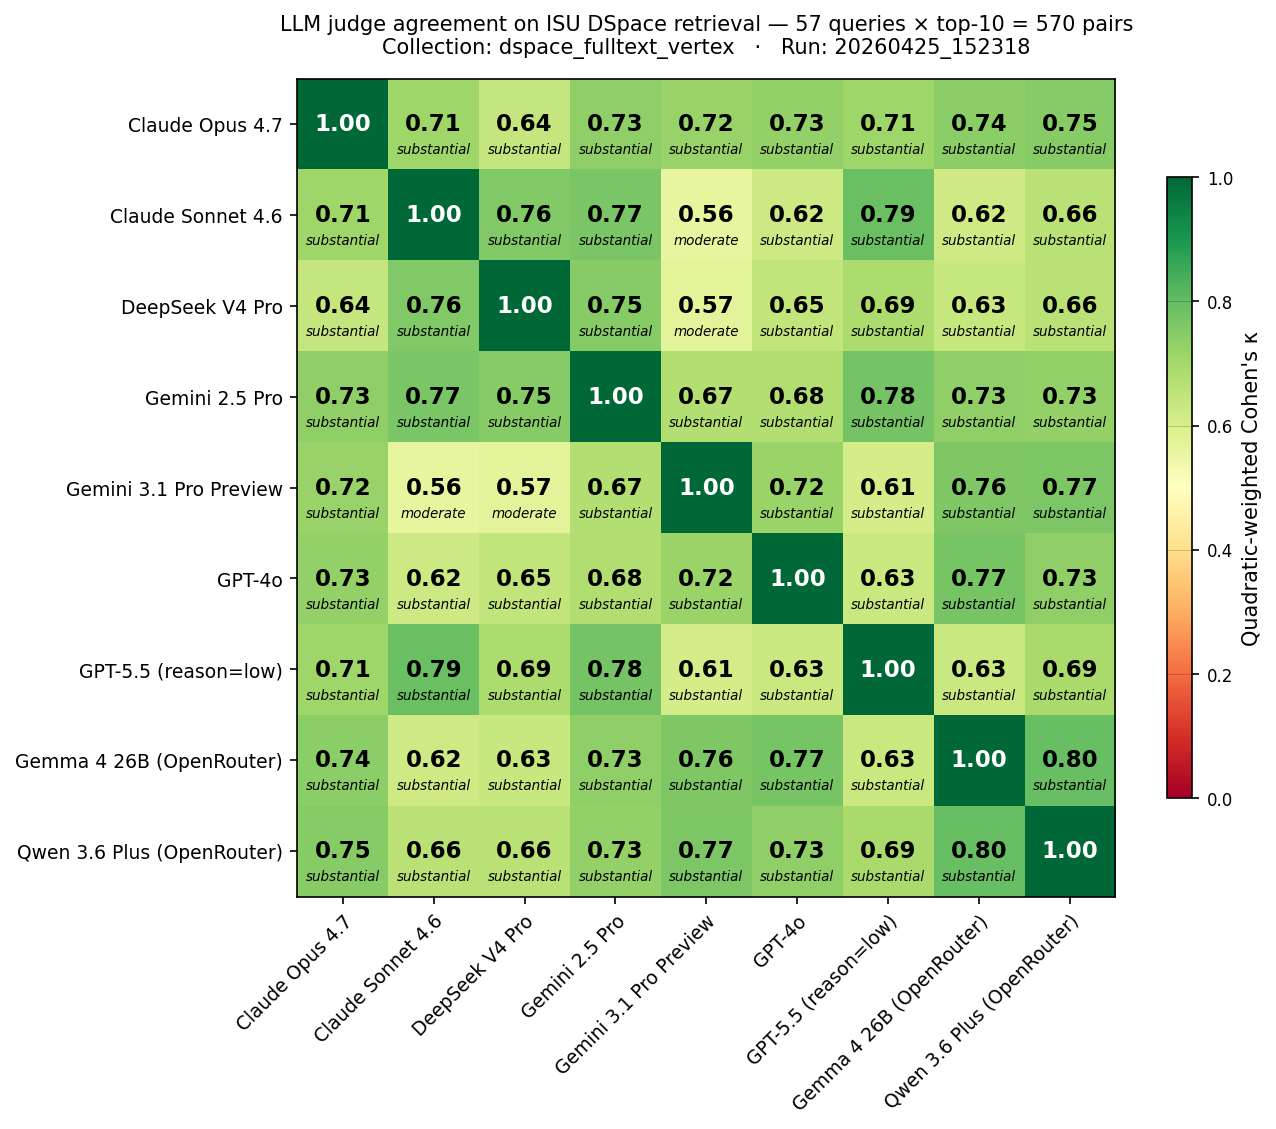
\includegraphics[width=0.92\linewidth]{kappa_matrix_9judge.png}
\caption{Pairwise quadratic-weighted Cohen's $\kappa$ on 570 ISU DSpace retrieval pairs. Two emergent calibration clusters; matrix-max $\kappa = 0.80$ between Qwen 3.6 Plus and Gemma 4 26B (cross-organization open-weight).}
\label{fig:kappa}
\end{figure}

\section{Findings (C1--C4)}\label{sec:findings}

\textbf{C1. Cross-family reasoning judges converge at $\kappa \geq 0.75$.} \textbf{Nine cross-family pairs} reach substantial-or-better $\kappa \geq 0.75$ (Fig.~\ref{fig:kappa}), spanning every pairwise combination of the five families---well above 0.4--0.6 typical \citep{rahmani2024judges} and the 0.60 unweighted baseline of \citet{thakur2025trecragsupport}. \textbf{DeepSeek V4 Pro joining the cluster makes a ``Western training data'' common-cause explanation less plausible,} and the pattern replicates across three independent ablation scales (5-, 7-, 9-judge) within run-to-run noise. The 9-judge ensemble achieves $\kappa = 0.49$ against published NIST qrels on TREC RAG 2024 (537 stratified-balanced pairs; Section~\ref{sec:validation}), so the convergence is not specific to our institutional corpus.

\textbf{C2. Within-family agreement is bounded by the cross-family ceiling.} Three of four within-family pairs are at or below the strongest cross-family commercial pair (0.79): Anthropic 0.71, OpenAI 0.63, Google-commercial 0.67. The fourth, cross-organization Open-weight (Qwen $\leftrightarrow$ Gemma 4 = 0.80), is the matrix maximum. \textbf{No commercial within-family pair dominates cross-family agreement}---at odds with self-preference findings on open-ended generation \citep{panickssery2024self}. Our companion 4-way extraction study reports within-family $\sim$2$\times$ cross-family on open-vocabulary tasks; the inversion under bounded ordinal judging suggests self-preference may be mediated by output-space boundedness rather than provider lineage (we discuss this hypothesis in Section~\ref{sec:limits}).

\textbf{C3. Open-weight judges produce the matrix-highest within-pair $\kappa$ and cluster with strict-mid commercial models.} Qwen $\leftrightarrow$ Gemma~4 = \textbf{0.80}---exceeds every commercial within-family pair and ties the cross-family reasoning ceiling. Both open-weight judges (mean 1.11--1.18) cluster with GPT-4o and Opus~4.7 (1.09--1.15) \textbf{not} with the reasoning-generous triad (1.63--1.68). At $\sim$USD~0.30 marginal cost via API routing, \textbf{an open-weight cross-organization pair achieves higher cross-validation $\kappa$ than the $\sim$USD~18 commercial 7-judge frontier}; we note that this measurement uses API routing rather than self-hosted inference, so on-prem economics are an extrapolation pending direct replication. External corroboration: Qwen and Gemma~4 both achieve \textbf{100\% coverage} on TREC RAG 2024 (better than 4 of 7 frontier judges), with individual $\kappa$ vs.\ human qrels of 0.41 each.

\textbf{C4. Open-source toolkit and disclosure template.} We release \texttt{eval\_llm\_judge.py} (multi-judge mode, ThreadPool fan-out), \texttt{validate\_against\_trec.py} (multi-corpus external-validation harness for TREC RAG 2024 / BEIR scifact / TREC-COVID), \texttt{fetch\_msmarco\_passages.py} (HF-streaming MS MARCO v2.1 passage extractor), the cross-run merge harness, the 57-query REFINE set, the rubric template, all 9 within-corpus per-judge JSONs (5{,}130 records), and the 9 external-validation JSONs (4{,}833 records).

\section{Mechanism (Summary)}\label{sec:mechanism}

\textbf{Decomposition of $\kappa$.} A joint-distribution decomposition into dispersion (the quadratic-disagreement weight, which appears in the $\kappa$ formula by construction) and effective rank (a singular-value summary of the 4$\times$4 confusion matrix) recovers $R^2 = 0.928$ across the 36 unique judge pairs. The high $R^2$ with dispersion is \textit{partly mathematical}---synthetic-pair simulation confirms $R^2 \approx 0.998$ in the limit purely from the $\kappa$ formula's weighting structure---so we present this as a \textbf{decomposition}, not as the discovery of a hidden empirical relationship. Marginal-distribution KL divergence \citep{kullback1951} gives $R^2 = 0.33$ as a coarser proxy. \textbf{The empirically interesting result is that structural factors (provider, reasoning-mode, model class) add $\leq 0.005$ incremental $R^2$ above the decomposition and are individually non-significant} (all $p > 0.18$)---descriptively consistent with full mediation in the spirit of \citet{baronkenny1986} and \citet{mackinnon2007}, though $n = 36$ limits the inferential strength. The \textbf{shared-tokenizer hypothesis is refuted}: Qwen $\leftrightarrow$ Gemma~4 vocabulary Jaccard $= 0.066$ (lowest in slate) yet $\kappa = 0.80$ (matrix-highest); convergence is at the decision-making layer, not the tokenizer. We use Cohen's $\kappa$ \citep{cohen1968} in its original quadratic-weighted formulation per \citet{fleiss1971} with Landis--Koch \citep{landis1977} bands. Full analysis with diagnostics, 36 confusion matrices, and per-pair tokenizer-overlap table: companion long version, \S6.

\section{External Validation Against NIST Human Qrels}\label{sec:validation}

To address single-corpus exposure, we replicated the 9-judge slate on \textbf{TREC RAG 2024} \citep{macavaney2025trec_rag} (537 stratified-balanced pairs from the official 20{,}283-pair NIST qrels, balanced 135/134/134/134 across labels 0/1/2/3, 86 queries; MS MARCO v2.1 passages extracted via HF-streaming filter from \texttt{drexalt/msmarco-2.1-segmented}).

\textbf{Results.} Per-judge $\kappa$ vs.\ human qrels ranges 0.40--0.55; \textbf{9-judge ensemble median $\kappa = 0.4941$}, \textbf{7-judge frontier-only $\kappa = 0.5187$} (open-weight broadens coverage, slightly lowers $\kappa$---a robustness/headline tradeoff). 5 of 9 judges hit $\kappa \geq 0.47$. Compared to \citet{thakur2025trecragsupport}'s GPT-4o $\kappa = 0.60$, our GPT-4o $= 0.41$---gap likely from sample (ours stratified-balanced; theirs natural-proportional), prompting, qrels version.

\textbf{Third-corpus replication on TREC-COVID} (300 biomedical-scientific pairs, BEIR-distributed) reaches 9-judge ensemble $\kappa = $ \textbf{0.3447} (fair-near-moderate), with Opus 4.7 leading at 0.53 and the frontier-7 subset at 0.4462; Qwen + Gemma 4 broaden coverage to 100\% but trail their TREC RAG 2024 numbers (0.32/0.27 vs.\ 0.41/0.40), indicating the robustness--headline-$\kappa$ tradeoff is content-domain dependent. \textbf{Coverage divergence is a content-domain reliability axis.} On TREC RAG 2024, Anthropic + OpenAI + Qwen + Gemma all return scores on \textbf{100\%} of pairs; \textbf{Gemini 3.1 Pro Preview 24\%, Gemini 2.5 Pro 17\%} (thinking-mode parse aborts on long web-domain passages), DeepSeek V4 Pro 40\%. On BEIR scifact (300 pairs, all-positive qrels---$\kappa$ undefined; 9-judge ensemble precision at $\geq 2$ = \textbf{65.7\%}, range 43--75\%), the same Gemini judges hit 60--86\%---reliability depends on content character. The \textbf{always-works 6-judge subset} ($\geq 95\%$ across all three external corpora) is Anthropic + OpenAI + Qwen + Gemma---\textbf{the 2 cheapest judges make this subset}. Validation pipeline replaces a per-institution IRB study ($\sim$\$1{,}500--3{,}000, 6--12 weeks) with public-NIST evidence ($\sim$\$56, $\sim$13~h). Per-corpus tables: \texttt{PUBLIC\_BENCHMARKS\_VALIDATION.md}.

\section{Limitations and Reproducibility}\label{sec:limits}

\textbf{Single internal corpus.} Within-pair $\kappa$ numbers (Fig.~\ref{fig:kappa}) are on ISU DSpace; the open-weight $\kappa$ ceiling is the most likely finding to drift across domains, though Section~\ref{sec:validation}'s TREC RAG 2024 result bounds the drift on judge-vs-human agreement. \textbf{Stratified vs.\ natural-distribution sampling.} Our 537-pair sample is balanced; \citet{thakur2025trecragsupport}'s was natural-distribution-proportional, so direct numerical comparison is not strictly apples-to-apples. \textbf{DSV4 Flash dropped} (OpenRouter 429). \textbf{Missing-data caveats.} Opus 4.7 returned None on 78/570 (13.7\%); Gemini 3.1 Prev on 390/570 (68.4\%); Gemini 2.5 Pro on 273/570 (47.9\%). Aggregate metrics treat None as 0; valid-only means place both Gemini judges within the strict-mid cluster (1.17 / 1.45) rather than as extreme outliers.

\textbf{Practitioner takeaway.} Judge interchangeability is a defensible default for reasoning-capable commercial judges; \textbf{calibration philosophy} (lenient vs.\ strict), not provider, is the axis on which retrieval verdicts shift; for sovereign-cloud deployments, the cross-organization open-weight pair achieves matrix-highest $\kappa$ at near-zero marginal cost.

\textbf{Reproducibility.} Single-command within-corpus replication: \texttt{py eval\_llm\_judge.py --collection <yours> --judge-preset p4-frontier}; $\sim$USD~18.30, $\sim$5.5\,h wall. Single-command external replication: \texttt{py validate\_against\_trec.py --corpus trec-rag-2024 --judge-preset p4-frontier --max-pairs 537}; $\sim$USD~35, $\sim$7.5\,h wall. Model versions pinned 2026-04-25. Code, data, and figures: \href{https://github.com/asukul/RAG-Eval-LLM-Judge}{github.com/asukul/RAG-Eval-LLM-Judge}. Targeting SIGIR Artifact Badging (Functional/Reusable). Companion long version contains full mechanism analysis, expanded validation tables, and 6 supplementary appendices.

\section*{Acknowledgments}

This work was conducted on the Iowa State University Digital Repository (DSpace); we thank the \textbf{ISU Library and Digital Initiatives team} for corpus access and the \textbf{ISU IT systems team} for the Qdrant deployment infrastructure. We thank the \textbf{Anthropic, OpenAI, Google DeepMind, DeepSeek, Alibaba, and Google (Gemma)} model teams for the model snapshots used here, and the \textbf{OpenRouter} team for the gateway that made cross-family API access economically feasible. Section~\ref{sec:validation} external validation uses the \textbf{NIST TREC RAG 2024} qrels \citep{macavaney2025trec_rag} and the MS MARCO v2.1 segmented corpus mirrored on Hugging Face by \texttt{drexalt/msmarco-2.1-segmented}. The BEIR scifact dataset is maintained by the \textbf{BEIR consortium} \citep{thakur2021beir}. API costs ($\sim$USD~56) were covered by personal research budget; we acknowledge the use of Claude Code as a coding assistant for harness implementation. Remaining errors are the author's.

\bibliographystyle{plainnat}
\bibliography{references}

\end{document}
